\documentclass{article}
\usepackage{hyperref}
\usepackage[utf8]{inputenc}
\usepackage[english]{babel}
\usepackage{amsmath}
\usepackage{todonotes}
\usepackage{siunitx}
\usepackage{float}
\sisetup{locale=DE}

\title{Computer Vision I - Sheet 2}
\author{ Jonas Otto\\ \href{mailto:jonas@jonasotto.com}{jonas@jonasotto.com} \and Dominik Authaler \\ 
\href{mailto:dominik.autaler@uni-ulm.de}{dominik.autlaler@uni-ulm.de}
}

\date{\today}

\begin{document}
\maketitle

\newpage

\section{Filter algebra}

\subsection{}
Given the filter $H = \left(\begin{array}{rrr}-1 & -2 & 0\\-2 & 0 & 2\\0 & 2 & 1\\\end{array}\right)$ and an Image $I \in [0, 255]$ the exercise arises the question what minimum and maximum output values this filter could create. Because all values in the image are positive, the maximum of 1275 is reached for a pixel region like $\left(\begin{array}{rrr}0 & 0 & 0\\0 & 0 & 255\\0 & 255 & 255\\\end{array}\right) $. Analogous the minimim value of -1275 is for instance reached in a pixel region like $\left(\begin{array}{rrr}255 & 255 & 0\\255 & 0 & 0\\0 & 0 & 0\\\end{array}\right)$.

\subsection{}
The source code used for this exercise is located in sh02ex01.m. The resulting images for task 2 are shown in the figures \ref{lenaGauss} and \ref{lenaR1}. For comparison purposes the original image is displayed in figure \ref{lena}. The filter H emphazises large constrasts along the diagonal from the bottom left to the top right corner. Because the filter only emphazises high constrasts, it belongs to the class of high-pass filters.
 
\begin{figure}[H]
	\begin{center}
		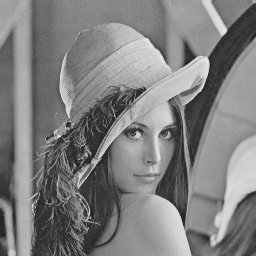
\includegraphics[width=\textwidth]{./images/lena.png}
		\caption{Original image} 
    \label{lena}
	\end{center}
\end{figure}

\begin{figure}[H]
	\begin{center}
		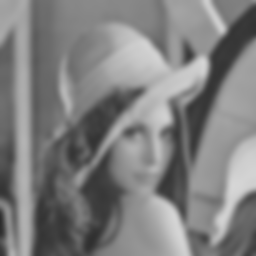
\includegraphics[width=\textwidth]{./images/imG.png}
		\caption{Gaussian kernel applied to lena.tiff} 
    \label{lenaGauss}
	\end{center}
\end{figure}

\begin{figure}[H]
	\begin{center}
		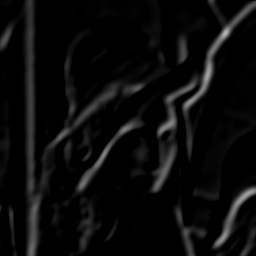
\includegraphics[width=\textwidth]{./images/imR1}
		\caption{Resulting image for $R_1 = I * G_{\sigma} * H$} 
    \label{lenaR1}
	\end{center}
\end{figure}

\subsection{}
The figures \ref{lenaH} to \ref{lenaDiff} show the results to task 3. Although the image shown in figure \ref{lenaDiff} looks quite dark, the sum over all pixels in the image is aproximately 31. Compared to the size of the image (256px $\times$ 256px) this number is so small, that one could argue that the error is coming from the small inaccuraries related to calculating with floating point numbers. 
Therefore the example shows the commutative property the convolution owns quite well. 

\begin{figure}[H]
	\begin{center}
		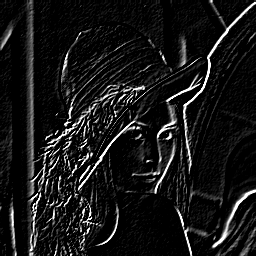
\includegraphics[width=\textwidth]{./images/imH.png}
		\caption{Filter H applied to lena.tiff}
    \label{lenaH}
	\end{center}
\end{figure}

\begin{figure}[H]
	\begin{center}
		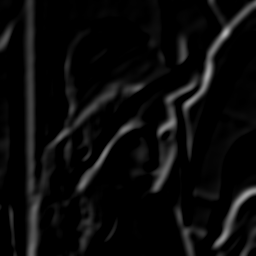
\includegraphics[width=\textwidth]{./images/imR2.png}
		\caption{Resulting image for $R_2 = I * H * G_{\sigma}$} 
    \label{lenaR2}
	\end{center}
\end{figure}

\begin{figure}[H]
	\begin{center}
		
\includegraphics[width=\textwidth]{./images/imDiff.png}
		\caption{Resulting image for $\left|R_1 - R_2\right|$} 
    \label{lenaDiff}
	\end{center}
\end{figure}

\clearpage
\section{Discrete Fourier Transform}
\subsection{}
Our implementation of the Discrete Fourier Transform can be found in the file fourier.m. Figure \ref{dft} shows the results of applying our DFT to the given signal.

\begin{figure}[H]
	\begin{center}
		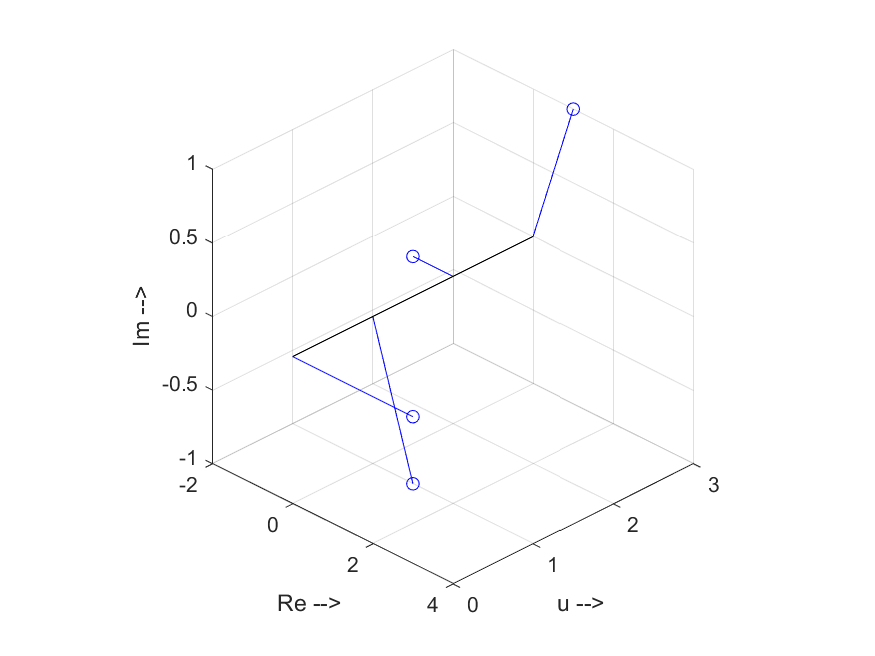
\includegraphics[width=\textwidth]{./images/Stemcomplex.png}
		\caption{Complex visualization of the results of the DFT} 
    \label{dft}
	\end{center}
\end{figure}

\subsection{}
Figure \ref{sin} shows the sine wave which corresponds to the vector at u = 1 in Figure \ref{dft}. Because this vector has both a real and an imaginary component not equal to zero it would also create a cosine wave. Both waves together would then represent this part in the original signal.
\begin{figure}[H]
	\begin{center}
		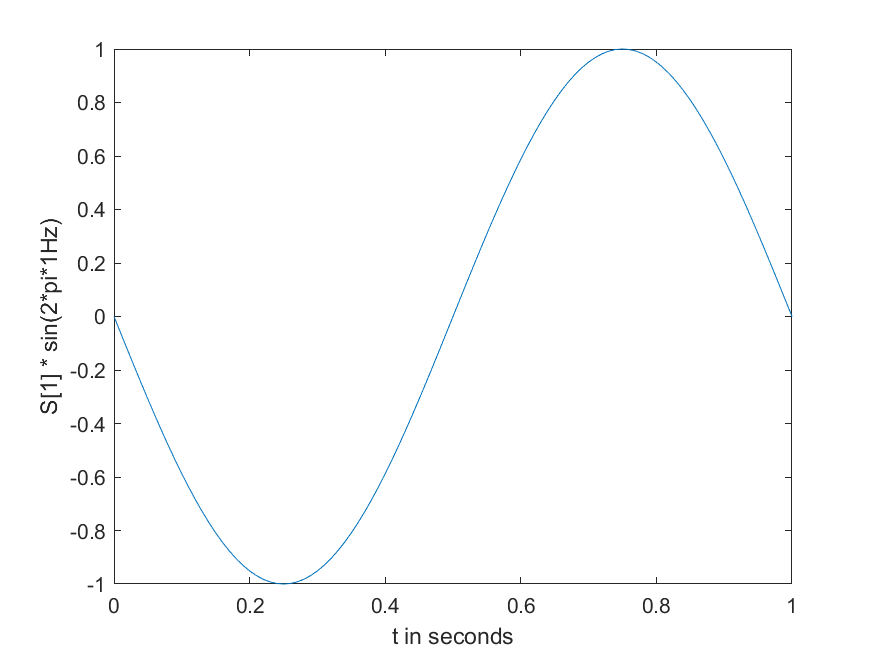
\includegraphics[width=\textwidth]{./images/Sinus.png}
		\caption{Sinus component of the complex value representing 1Hz} 
    \label{sin}
	\end{center}
\end{figure}

\subsection{}
The source code used for this task can be found in the file ifourier.m.

\subsection{}
Figure \ref{results} shows the results gained from task a) to c). Because the third value of the reconstructed signal is not exact zero but of the magnitude $10^{-16}$ Matlab expands the vertical axis in the third plot a bit into the negative direction. Besides this small difference, the reconstructed signal looks the same compared to the orignal signal. Because our signal was sampled with a sampling frequency of 4$\si{Hz}$ and the sampled signal has 4 points, the frequency resolution of the frequency spectrum is $\frac{4\si{Hz}}{4} = 1\si{Hz}$.

\begin{figure}[H]
	\begin{center}
		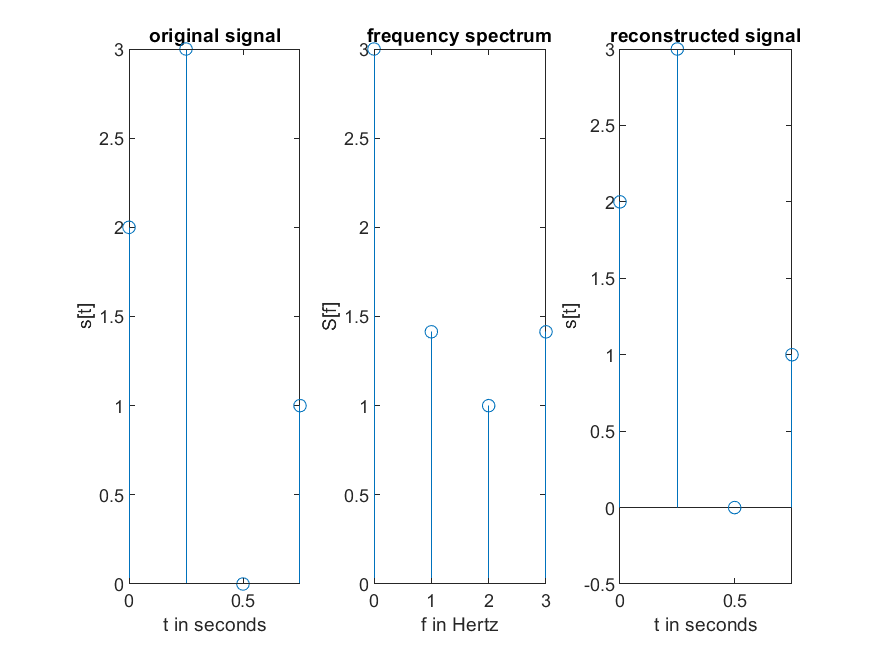
\includegraphics[width=\textwidth]{./images/figure_d.png}
		\caption{Plots showing results from task a) to c)} 
    \label{results}
	\end{center}
\end{figure}

\clearpage
\section{Fourier Transform for Image Quality Assessment}
The source used to create the figures shown in this section can be found in the Matlab script sh03ex03.m.
Figure \ref{ex03} shows the original images together with their already high-pass filtered frequency spectra calculated with fft2. The spectra have been shifted using fftshift. Figure \ref{ex03_highpass} shows the high-pass filter which was used. According to the exercise we set sigma to the half of the image height. In a first try we used the rule for the filter size given in exercise 1. But this lead to a filter which was much bigger than the original image. Therefore we scaled it so that it fits to the image and can be directly applied in the frequency domain by multiplication. Above the images one can find the energy calculated for this image. The left image is the sharp one, thus we expected the energy of it's filtered spectrum being higher than in the filtered spectrum of the other image. Our calculation proves what we expected, the energy of the left spectrum is about twice the energy of the right spectrum. 

\begin{figure}[H]
	\begin{center}
		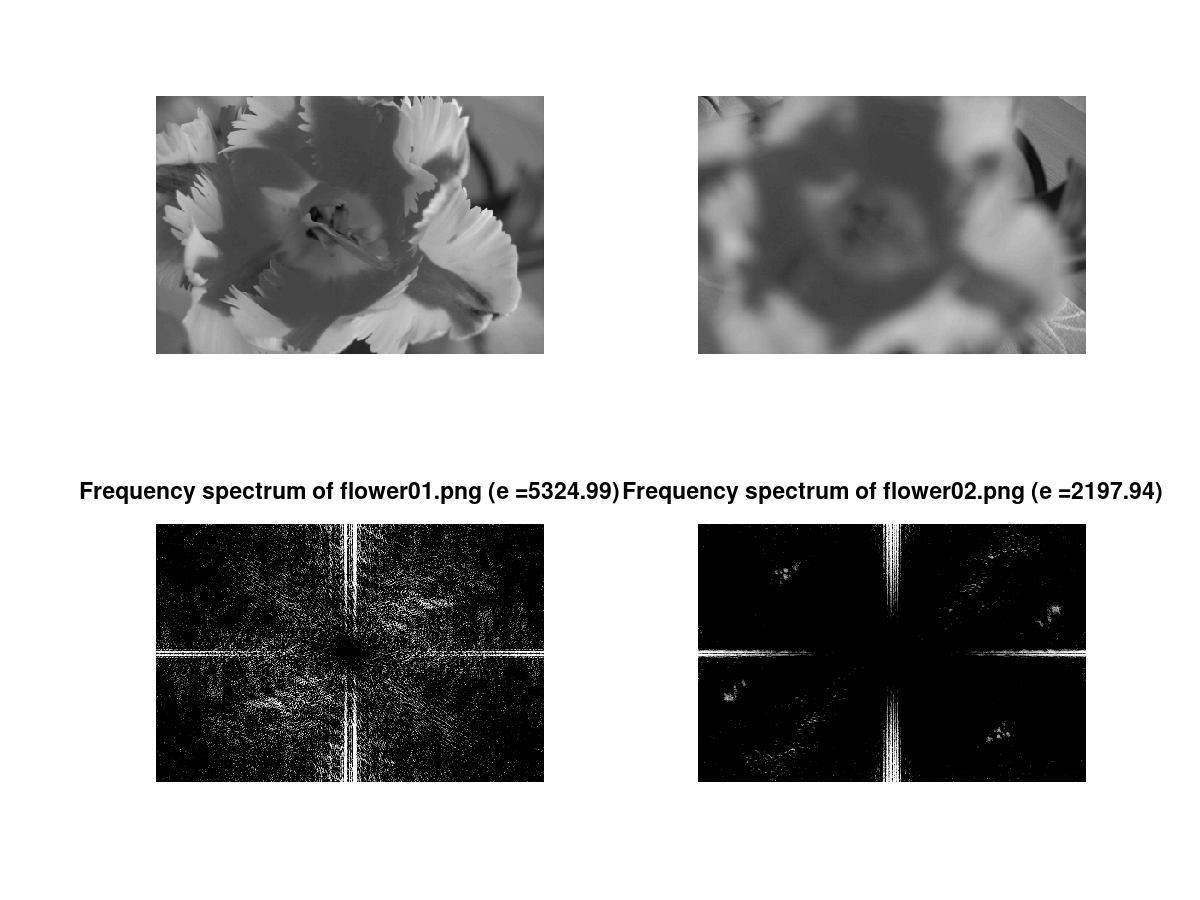
\includegraphics[width=\textwidth]{./images/ex03_1.png}
		\caption{Original images and their frequency spectra}
    \label{ex03}
	\end{center}
\end{figure}

\begin{figure}[H]
	\begin{center}
		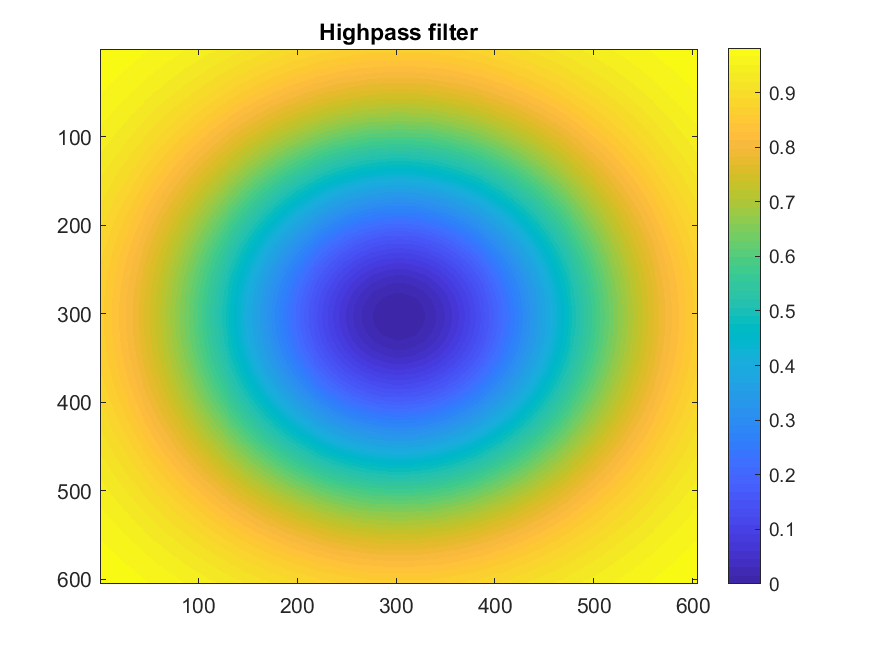
\includegraphics[width=\textwidth]{./images/ex03_2.png}
    \label{ex03_highpass}
		\caption{Highpass filter} 
	\end{center}
\end{figure}

\end{document}
